\documentclass[12pt]{article}

% --- Mandatory Packages ---
\usepackage{amsmath}
\usepackage{amssymb}
\usepackage{amsthm}
\usepackage{geometry}
\usepackage{tikz}
\usetikzlibrary{arrows.meta, positioning, shapes}
\usepackage{mathrsfs}
\usepackage{mathtools}
\usepackage{xcolor}

% --- Page Setup ---
\geometry{letterpaper, margin=1in}

% --- Theorem Environments ---
\newtheorem{theorem}{Theorem}[section]
\newtheorem{lemma}[theorem]{Lemma}
\newtheorem{proposition}[theorem]{Proposition}
\newtheorem{corollary}[theorem]{Corollary}
\theoremstyle{definition}
\newtheorem{definition}{Definition}[section]
\newtheorem{axiom}{Axiom}[section]
\newtheorem{example}{Example}[section]
\theoremstyle{remark}
\newtheorem{remark}{Remark}[section]
\newtheorem{fallacy}{Fallacy}[section]

% --- Title Information ---
\title{Homework 4.6: Proofs Involving Cartesian Products of Sets}
\author{Tashfeen Omran}
\date{September 2026}

\begin{document}

\maketitle
\tableofcontents
\newpage

% ==============================================================================
% PART 1: Comprehensive Introduction, Context, and Prerequisites
% ==============================================================================
\section{Part 1: Comprehensive Introduction, Context, and Prerequisites}

\subsection{Historical Context and Motivation}
The concept of the Cartesian product is named after the French mathematician and philosopher René Descartes. By formulating analytic geometry in the 17th century, Descartes created a bridge between algebra and Euclidean geometry. He showed that points in a plane could be represented as ordered pairs of real numbers, mapping geometric space to the set $\mathbb{R} \times \mathbb{R}$. In the late 19th and early 20th centuries, pioneers like Georg Cantor and Ernst Zermelo rigorously formalized set theory, recognizing the Cartesian product not just as a coordinate grid, but as a foundational mechanism for constructing new, complex sets from simpler ones. In modern mathematics, Cartesian products are the logical bedrock upon which relations, functions, state-spaces, and joint probability distributions are explicitly built.

\subsection{Core Concepts \& Axioms}
At the heart of the Cartesian product is the notion of order. Unlike a standard set $\{a, b\}$, where $\{a, b\} = \{b, a\}$, an \textbf{ordered pair} $(a, b)$ strictly enforces sequence: $(a, b) = (c, d)$ if and only if $a = c$ and $b = d$. Formally, within Zermelo-Fraenkel (ZF) set theory, an ordered pair is defined via the Kuratowski definition: 
\[ (a, b) \coloneqq \{\{a\}, \{a, b\}\} \]

\begin{definition}[Cartesian Product]
Let $A$ and $B$ be sets. The Cartesian product of $A$ and $B$, denoted $A \times B$, is the set of all ordered pairs $(a, b)$ where $a \in A$ and $b \in B$. Expressed in set-builder notation:
\[ A \times B = \{(a, b) : a \in A \text{ and } b \in B\} \]
\end{definition}

\subsection{Intuition and Set-Theoretic Foundations}
Geometrically, if $A$ represents a horizontal axis and $B$ represents a vertical axis, $A \times B$ represents the grid of intersections. If $A$ and $B$ are finite, the cardinality of their Cartesian product is strictly multiplicative: $|A \times B| = |A| \cdot |B|$. A critical foundational property is that if either $A$ or $B$ is empty, it is impossible to form an ordered pair. Thus, $A \times B = \emptyset$ if and only if $A = \emptyset$ or $B = \emptyset$.

\subsection{Key Theorems and Equivalences}
\begin{itemize}
    \item \textbf{Distributivity over Union:} $A \times (B \cup C) = (A \times B) \cup (A \times C)$
    \item \textbf{Distributivity over Intersection:} $A \times (B \cap C) = (A \times B) \cap (A \times C)$
    \item \textbf{Subset Preservation:} If $A \subseteq C$ and $B \subseteq D$, then $A \times B \subseteq C \times D$
    \item \textbf{Difference Distribution:} $A \times (B - C) = (A \times B) - (A \times C)$
\end{itemize}

\subsection{Prerequisites}
To fully master this section, the student must be comfortable with:
\begin{enumerate}
    \item \textbf{Element-Chasing Proofs:} Choosing an arbitrary element $x \in S$ to show $S \subseteq T$.
    \item \textbf{Bi-conditional Logic:} Proving $P \iff Q$ by showing $P \implies Q$ and $Q \implies P$.
    \item \textbf{Power Sets:} Understanding that $\mathcal{P}(A)$ is the set of all subsets of $A$.
    \item \textbf{Contrapositive \& Contradiction:} Utilizing $\sim Q \implies \sim P$ when direct proofs involving empty sets are computationally elusive.
\end{enumerate}

\newpage
% ==============================================================================
% PART 2: Detailed Homework Solutions
% ==============================================================================
\section{Part 2: Detailed Homework Solutions (Rigorous Proofs \& Computations)}

\textit{Note: Per the strategic optimization protocol, problems have been selectively chosen to guarantee comprehensive coverage of every distinct problem archetype (Computations, Set Algebra Equivalence, Subsets, and Counterexamples/Falsifications) with at least two problems per type.}

\subsection{Problem Archetype 1: Computations and Power Sets}

\textbf{Problem 4.60:} For $A = \{x, y\}$, determine $A \times \mathcal{P}(A)$.

\begin{proof}[Solution]
First, we compute the power set of $A$, which is the set of all subsets of $A$.
Since $|A| = 2$, $|\mathcal{P}(A)| = 2^2 = 4$.
\[ \mathcal{P}(A) = \{\emptyset, \{x\}, \{y\}, \{x, y\}\} \]
By the definition of the Cartesian product, $A \times \mathcal{P}(A)$ consists of all ordered pairs where the first element belongs to $A$ and the second element belongs to $\mathcal{P}(A)$.
\begin{align*}
A \times \mathcal{P}(A) &= \{ (a, B) : a \in A, B \in \mathcal{P}(A) \} \\
&= \{ (x, \emptyset), (x, \{x\}), (x, \{y\}), (x, \{x, y\}), \\
&\quad \ \ (y, \emptyset), (y, \{x\}), (y, \{y\}), (y, \{x, y\}) \}
\end{align*}
This contains exactly $|A| \cdot |\mathcal{P}(A)| = 2 \cdot 4 = 8$ elements, which confirms the computation is complete.
\end{proof}

\vspace{0.5cm}

\textbf{Problem 4.61:} For $A = \{1\}$ and $B = \{2\}$, determine $\mathcal{P}(A \times B)$ and $\mathcal{P}(A) \times \mathcal{P}(B)$.

\begin{proof}[Solution]
First, compute the Cartesian product $A \times B$:
\[ A \times B = \{(1, 2)\} \]
The power set of $A \times B$ is the set of all subsets of $A \times B$. Since $|A \times B| = 1$, $|\mathcal{P}(A \times B)| = 2^1 = 2$.
\[ \mathcal{P}(A \times B) = \{\emptyset, \{(1, 2)\}\} \]

Next, we compute $\mathcal{P}(A) \times \mathcal{P}(B)$. We find the individual power sets first:
\[ \mathcal{P}(A) = \{\emptyset, \{1\}\} \]
\[ \mathcal{P}(B) = \{\emptyset, \{2\}\} \]
The Cartesian product of these two power sets yields:
\begin{align*}
\mathcal{P}(A) \times \mathcal{P}(B) &= \{ (X, Y) : X \in \mathcal{P}(A), Y \in \mathcal{P}(B) \} \\
&= \{ (\emptyset, \emptyset), (\emptyset, \{2\}), (\{1\}, \emptyset), (\{1\}, \{2\}) \}
\end{align*}
This highlights a crucial conceptual difference: $\mathcal{P}(A \times B)$ contains sets of ordered pairs, whereas $\mathcal{P}(A) \times \mathcal{P}(B)$ contains ordered pairs of sets.
\end{proof}

\subsection{Problem Archetype 2: Empty Sets and Bi-conditional Logic}

\textbf{Problem 4.62:} Let $A$ and $B$ be sets. Prove that $A \times B = \emptyset$ if and only if $A = \emptyset$ or $B = \emptyset$.

\begin{proof}[Proof by Contrapositive (Both Directions)]
We must prove the biconditional statement $(A \times B = \emptyset) \iff (A = \emptyset \lor B = \emptyset)$. We will prove both directions using the contrapositive.

\textbf{Direction 1 ($\impliedby$):} Prove $(A = \emptyset \lor B = \emptyset) \implies (A \times B = \emptyset)$.
The contrapositive is: $(A \times B \neq \emptyset) \implies (A \neq \emptyset \land B \neq \emptyset)$.
Assume $A \times B \neq \emptyset$. By definition, there exists at least one element in $A \times B$. Let this element be an ordered pair $(x, y)$. By the definition of the Cartesian product, $(x, y) \in A \times B$ implies that $x \in A$ and $y \in B$. Because $A$ contains the element $x$, $A \neq \emptyset$. Because $B$ contains the element $y$, $B \neq \emptyset$. Thus, $A \neq \emptyset \land B \neq \emptyset$. The contrapositive holds, thus the original implication is true.

\textbf{Direction 2 ($\implies$):} Prove $(A \times B = \emptyset) \implies (A = \emptyset \lor B = \emptyset)$.
The contrapositive is: $(A \neq \emptyset \land B \neq \emptyset) \implies (A \times B \neq \emptyset)$.
Assume $A \neq \emptyset$ and $B \neq \emptyset$. Since $A$ is not empty, there exists some $a \in A$. Since $B$ is not empty, there exists some $b \in B$. By the definition of the Cartesian product, the ordered pair $(a, b) \in A \times B$. Since $A \times B$ contains at least one element, $A \times B \neq \emptyset$. The contrapositive holds, thus the original implication is true.

Since both implications are true, the biconditional $A \times B = \emptyset \iff A = \emptyset \lor B = \emptyset$ is proven.
\end{proof}

\vspace{0.5cm}

\textbf{Problem 4.65:} Let $A$, $B$, and $C$ be nonempty sets. Prove that $A \times C \subseteq B \times C$ if and only if $A \subseteq B$.

\begin{proof}[Direct Proof]
Assume $A$, $B$, and $C$ are nonempty. We prove both directions of the biconditional.

\textbf{Direction 1 ($\impliedby$):} Assume $A \subseteq B$. We want to show $A \times C \subseteq B \times C$.
Let $(x, y) \in A \times C$ be an arbitrary element. By definition, $x \in A$ and $y \in C$. Since $A \subseteq B$, the fact that $x \in A$ implies $x \in B$. Therefore, we have $x \in B$ and $y \in C$, which means $(x, y) \in B \times C$. Since $(x,y)$ was arbitrary, $A \times C \subseteq B \times C$.

\textbf{Direction 2 ($\implies$):} Assume $A \times C \subseteq B \times C$. We want to show $A \subseteq B$.
Let $a \in A$ be an arbitrary element. We must show $a \in B$. Since we are given that $C$ is a nonempty set, there exists at least one element $c \in C$. Because $a \in A$ and $c \in C$, the ordered pair $(a, c) \in A \times C$. By our assumption, $A \times C \subseteq B \times C$, so it follows that $(a, c) \in B \times C$. By the definition of the Cartesian product, this means the first coordinate $a$ must belong to $B$ (and $c \in C$). Thus, $a \in B$. Since $a$ was an arbitrary element of $A$, we conclude $A \subseteq B$.

Both directions are proven.
\end{proof}

\subsection{Problem Archetype 3: Set Algebra Equivalences}

\textbf{Problem 4.67:} Let $A$, $B$, and $C$ be sets. Prove that $A \times (B \cap C) = (A \times B) \cap (A \times C)$.

\begin{proof}[Direct Proof (Series of Equivalences)]
We will prove this equality by demonstrating that an arbitrary ordered pair $(x,y)$ belongs to the left-hand side if and only if it belongs to the right-hand side. Let $(x,y)$ be an arbitrary ordered pair.
\begin{align*}
(x, y) \in A \times (B \cap C) &\iff x \in A \land y \in (B \cap C) \quad &&\text{(Def. of Cartesian Product)} \\
&\iff x \in A \land (y \in B \land y \in C) \quad &&\text{(Def. of Intersection)} \\
&\iff (x \in A \land x \in A) \land (y \in B \land y \in C) \quad &&\text{(Idempotence of $\land$)} \\
&\iff (x \in A \land y \in B) \land (x \in A \land y \in C) \quad &&\text{(Associativity/Commutativity)} \\
&\iff (x, y) \in A \times B \land (x, y) \in A \times C \quad &&\text{(Def. of Cartesian Product)} \\
&\iff (x, y) \in (A \times B) \cap (A \times C) \quad &&\text{(Def. of Intersection)}
\end{align*}
Because every step is a logical biconditional ($\iff$), the two sets are strictly equal.
\end{proof}

\vspace{0.5cm}

\textbf{Problem 4.68:} Let $A$, $B$, $C$, and $D$ be sets. Prove that $(A \times B) \cap (C \times D) = (A \cap C) \times (B \cap D)$.

\begin{proof}[Direct Proof (Series of Equivalences)]
We employ the same strategy as the previous proof. Let $(x,y)$ be an arbitrary ordered pair.
\begin{align*}
(x, y) \in (A \times B) \cap (C \times D) &\iff (x, y) \in A \times B \land (x, y) \in C \times D \\
&\iff (x \in A \land y \in B) \land (x \in C \land y \in D) \\
&\iff (x \in A \land x \in C) \land (y \in B \land y \in D) \quad &&\text{(Rearranging terms)} \\
&\iff x \in (A \cap C) \land y \in (B \cap D) \\
&\iff (x, y) \in (A \cap C) \times (B \cap D)
\end{align*}
Since the logic holds biconditionally, the sets are identically equal. 
\end{proof}

\subsection{Problem Archetype 4: Counterexamples and Subtleties}

\textbf{Problem 4.66:} Result 4.23 states that if $A, B, C, D$ are sets such that $A \subseteq C$ and $B \subseteq D$, then $A \times B \subseteq C \times D$.
(a) Show that the converse of Result 4.23 is false.
(b) Under what added hypothesis is the converse true? Prove your assertion.

\begin{proof}[Solution to (a): Counterexample]
The converse states: "If $A \times B \subseteq C \times D$, then $A \subseteq C$ and $B \subseteq D$."
To show this is false, we must provide a counterexample where the premise is true but the conclusion is false.
Let $A = \emptyset$, $B = \{1\}$, $C = \{2\}$, and $D = \{3\}$.
We evaluate the premise: $A \times B = \emptyset \times \{1\} = \emptyset$.
The right side is $C \times D = \{2\} \times \{3\} = \{(2,3)\}$.
Since the empty set is a subset of every set, $\emptyset \subseteq \{(2,3)\}$ is trivially true. Thus, the premise $A \times B \subseteq C \times D$ holds.
However, evaluate the conclusion: Is $B \subseteq D$? $\{1\} \not\subseteq \{3\}$. The conclusion is false. Therefore, the converse is false.
\end{proof}

\begin{proof}[Solution to (b): Added Hypothesis]
The failure in part (a) occurred because an empty Cartesian product trivially fulfills subset relations without restricting the individual coordinate sets. To fix this, we add the hypothesis: $\mathbf{A \times B \neq \emptyset}$ (which, by Problem 4.62, implies $A \neq \emptyset$ and $B \neq \emptyset$).

\textbf{New Claim:} If $A \times B \neq \emptyset$ and $A \times B \subseteq C \times D$, then $A \subseteq C$ and $B \subseteq D$.

Let $A \times B \neq \emptyset$ and $A \times B \subseteq C \times D$. We first show $A \subseteq C$. 
Let $a \in A$. Since $A \times B \neq \emptyset$, we know $B \neq \emptyset$. Thus, there exists some element $b \in B$. 
Form the ordered pair $(a, b)$. Since $a \in A$ and $b \in B$, $(a, b) \in A \times B$. 
By our subset assumption, $(a, b) \in C \times D$. By the definition of the Cartesian product, this means $a \in C$ and $b \in D$. 
Since $a \in C$ for any arbitrary $a \in A$, we have $A \subseteq C$.

By an identical symmetric argument, selecting an arbitrary $y \in B$ and utilizing some $x \in A$, we construct $(x, y) \in A \times B \subseteq C \times D \implies y \in D$, which yields $B \subseteq D$.
\end{proof}

\vspace{0.5cm}

\textbf{Problem 4.70:} Let $A$ and $B$ be sets. Show, in general, that $\overline{A \times B} \neq \bar{A} \times \bar{B}$.

\begin{proof}[Counterexample]
Let $U = \{1, 2\}$ be the universal set for our coordinates. The universal set for Cartesian products of these sets is therefore $U \times U = \{(1,1), (1,2), (2,1), (2,2)\}$.
Let $A = \{1\}$ and $B = \{1\}$.
We compute the left-hand side, $\overline{A \times B}$:
\[ A \times B = \{(1, 1)\} \]
\[ \overline{A \times B} = (U \times U) - (A \times B) = \{(1,2), (2,1), (2,2)\} \]
Next, we compute the right-hand side, $\bar{A} \times \bar{B}$:
\[ \bar{A} = U - A = \{2\} \]
\[ \bar{B} = U - B = \{2\} \]
\[ \bar{A} \times \bar{B} = \{2\} \times \{2\} = \{(2, 2)\} \]
Comparing the two sets:
\[ \{(1,2), (2,1), (2,2)\} \neq \{(2,2)\} \]
Thus, $\overline{A \times B} \neq \bar{A} \times \bar{B}$.
\end{proof}

\newpage
% ==============================================================================
% PART 3: In-Depth Analysis of Problems and Techniques
% ==============================================================================
\section{Part 3: In-Depth Analysis of Problems and Techniques}

\subsection{A) Problem Types and Logical Strategies}
The problems in this section naturally segment into several distinct categories:
\begin{enumerate}
    \item \textbf{Element-Chasing Subsets/Equality (e.g., 4.67, 4.68):} The dominant strategy here is translating set-theoretic notation into logical connectives (AND $\land$, OR $\lor$) inside an arbitrary ordered pair. By establishing a chain of logically equivalent statements ($\iff$), one proves equality strictly and concisely without needing separate subsets proofs for each direction.
    \item \textbf{Emptiness and Contrapositive Proofs (e.g., 4.62, 4.66):} A Cartesian product relies entirely on the existence of elements in \textit{both} constituent sets. Direct proofs involving $\emptyset$ are awkward because you cannot select an element. The strategy is to use the \textbf{contrapositive}: assume sets are non-empty so that you can invoke an explicit element $x \in A$.
    \item \textbf{Falsification via Counterexample (e.g., 4.66a, 4.70):} When asked to show a general statement is false, the strategy is to seek the boundary cases. The empty set $\emptyset$ is the universally most powerful tool for falsifying Cartesian assertions.
\end{enumerate}

\subsection{B) Key Analytical and Logical Manipulations}
\begin{itemize}
    \item \textbf{Tuple Unpacking:} The transition from $(x, y) \in (A \times B) \cap (C \times D)$ to $(x, y) \in A \times B \land (x, y) \in C \times D$. Breaking the composite object into fundamental logical propositions is the mechanism that allows basic logic rules (like commutativity of $\land$) to solve the problem.
    \item \textbf{Idempotence trick:} In problem 4.67, we used the fact that $x \in A$ is logically equivalent to $(x \in A \land x \in A)$. This artificial "duplication" of the premise allowed us to perfectly distribute the terms into the final structure $(x \in A \land y \in B) \land (x \in A \land y \in C)$.
\end{itemize}

% ==============================================================================
% PART 4: "Cheatsheet", Visuals, and Tips for Success
% ==============================================================================
\section{Part 4: "Cheatsheet", Visuals, and Tips for Success}

\subsection{Theorems \& Equivalences Cheatsheet}
\begin{itemize}
    \item $A \times (B \cup C) = (A \times B) \cup (A \times C)$
    \item $A \times (B \cap C) = (A \times B) \cap (A \times C)$
    \item $(A \times B) \cap (C \times D) = (A \cap C) \times (B \cap D)$
    \item $(A \subseteq B \land C \subseteq D) \implies A \times C \subseteq B \times D$
    \item $A \times B = \emptyset \iff (A = \emptyset \lor B = \emptyset)$
\end{itemize}

\subsection{Visual: Intersection of Cartesian Products (Problem 4.68)}
The following diagram provides geometric intuition for the proof of $(A \times B) \cap (C \times D) = (A \cap C) \times (B \cap D)$.

\vspace{0.5cm}
\begin{center}
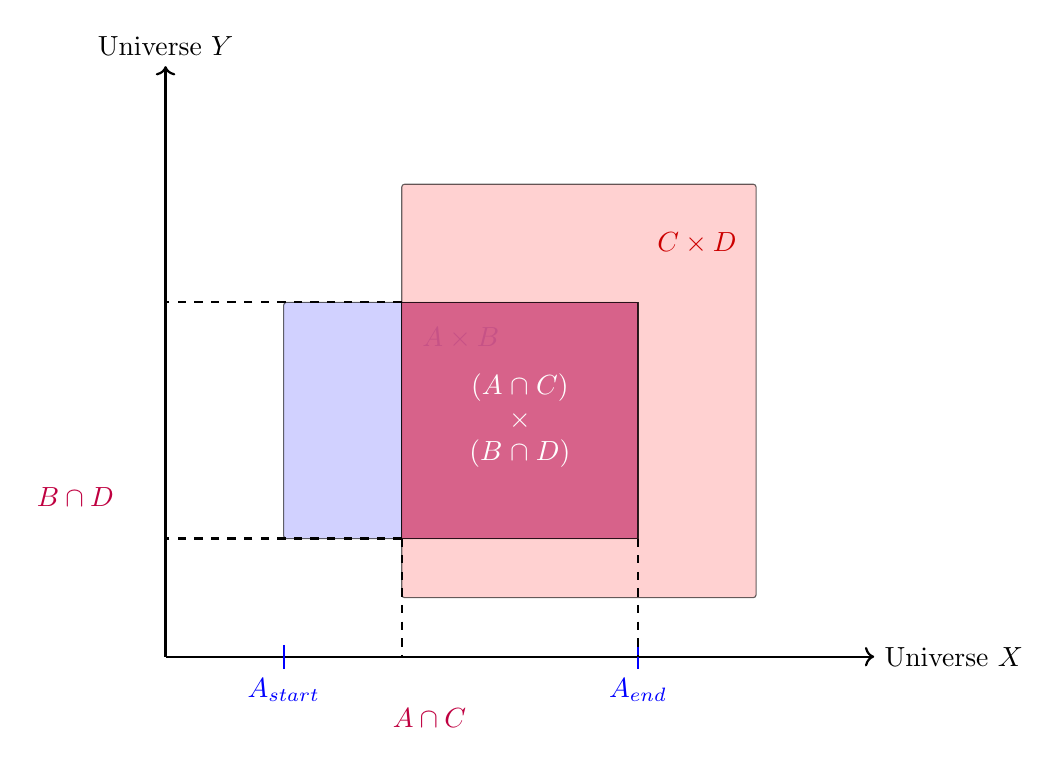
\begin{tikzpicture}[scale=1.5]
    % Axes
    \draw[thick, ->] (0,0) -- (6,0) node[right] {Universe $X$};
    \draw[thick, ->] (0,0) -- (0,5) node[above] {Universe $Y$};
    
    % A x B
    \draw[fill=blue!30, opacity=0.6, rounded corners=1pt] (1,1) rectangle (4,3);
    \node[blue!80!black, font=\bfseries] at (2.5, 2.7) {$A \times B$};
    \draw[blue, thick] (1,0.1) -- (1,-0.1) node[below] {$A_{start}$};
    \draw[blue, thick] (4,0.1) -- (4,-0.1) node[below] {$A_{end}$};
    
    % C x D
    \draw[fill=red!30, opacity=0.6, rounded corners=1pt] (2,0.5) rectangle (5,4);
    \node[red!80!black, font=\bfseries] at (4.5, 3.5) {$C \times D$};
    
    % Intersection
    \draw[fill=purple!70, opacity=0.8] (2,1) rectangle (4,3);
    \node[white, font=\bfseries, text width=2cm, align=center] at (3, 2) {$(A \cap C)$ \\ $\times$ \\ $(B \cap D)$};
    
    % Axis projections for intersection
    \draw[dashed, thick] (2,1) -- (2,0) node[below=15pt, xshift=10pt, font=\bfseries, purple] {$A \cap C$};
    \draw[dashed, thick] (4,1) -- (4,0);
    
    \draw[dashed, thick] (2,1) -- (0,1) node[left=15pt, yshift=15pt, font=\bfseries, purple] {$B \cap D$};
    \draw[dashed, thick] (2,3) -- (0,3);
\end{tikzpicture}
\end{center}
\vspace{0.5cm}

\subsection{Pitfalls \& Fallacies}
\begin{fallacy}[The Distribution over Product Error]
Assuming that $(A \cup B) \times (C \cup D) = (A \times C) \cup (B \times D)$. \textbf{This is FALSE.} The left side contains cross-terms like $A \times D$ and $B \times C$. The correct formula is $(A \cup B) \times (C \cup D) = (A \times C) \cup (A \times D) \cup (B \times C) \cup (B \times D)$.
\end{fallacy}
\begin{fallacy}[The Complement Error]
Assuming $\overline{A \times B} = \bar{A} \times \bar{B}$. As shown in Problem 4.70, $\overline{A \times B} = (\bar{A} \times B) \cup (A \times \bar{B}) \cup (\bar{A} \times \bar{B})$.
\end{fallacy}

% ==============================================================================
% PART 5: Conceptual Synthesis and The "Big Picture"
% ==============================================================================
\section{Part 5: Conceptual Synthesis and The "Big Picture"}

\subsection{Thematic Connections}
The central theme of this chapter is \textit{extending unary set structures to binary relations}. Prior to this, sets were merely unstructured bins of objects. The Cartesian product introduces \textit{coordinates}. This is mathematically equivalent to the jump from points on a 1D number line to a 2D Euclidean plane. 

\subsection{Forward and Backward Links}
\begin{itemize}
    \item \textbf{Backward Link:} This concept logically extends the basic axioms of set operations (Union, Intersection, Complement) governed by De Morgan's Laws into higher dimensions. 
    \item \textbf{Forward Link:} The Cartesian product is the absolute prerequisite for Defining a \textbf{Relation}. Any relation $R$ from set $A$ to set $B$ is formally defined merely as a subset $R \subseteq A \times B$. From there, a \textbf{Function} is defined as a specific type of relation. Thus, Calculus, Linear Algebra, and Differential Equations are all inherently operating on subsets of Cartesian products. Furthermore, in measure theory, constructing a measure on a product space $X \times Y$ (product measure) is essential for integrating functions of multiple variables (Fubini's Theorem).
\end{itemize}

% ==============================================================================
% PART 6: Abstract Real-World Modeling (AI, ML, & Quant Finance)
% ==============================================================================
\section{Part 6: Abstract Real-World Modeling (AI, ML, \& Quant Finance)}

Abstract Cartesian products are strictly embedded in advanced stochastic and deterministic modeling in modern technology and finance.

\subsection{Concrete Scenarios}
\begin{enumerate}
    \item \textbf{Markov Decision Processes (Reinforcement Learning):} In AI, an agent navigating an environment evaluates its choices using a transition probability model. If the environment has a state space $\mathcal{S}$ and an action space $\mathcal{A}$, the agent's policy and transitions act upon the Cartesian product $\mathcal{S} \times \mathcal{A}$. A reward function is strictly a mapping $R: \mathcal{S} \times \mathcal{A} \to \mathbb{R}$.
    \item \textbf{Copulas in Quantitative Finance (Joint Probability Spaces):} To price a complex multi-asset derivative (like a collateralized debt obligation or a basket option), quants cannot just look at asset $A$ and asset $B$ independently. They must define a joint probability measure $\mathbb{P}$ on the product $\sigma$-algebra $\mathcal{F}_A \otimes \mathcal{F}_B$ defined over the Cartesian product space $\Omega_A \times \Omega_B$. 
\end{enumerate}

\subsection{Model Problem Setup: Joint Asset Dynamics in Arbitrage Theory}
Let us rigorously model the joint behavior of two underlying assets $S_1$ and $S_2$ in a quantitative finance framework using continuous-time stochastic processes. 
Let $(\Omega_1, \mathcal{F}_1, \mathbb{P}_1)$ and $(\Omega_2, \mathcal{F}_2, \mathbb{P}_2)$ be two probability spaces modeling the intrinsic, independent randomness of asset 1 and asset 2. 

To model a portfolio containing both, we establish the Cartesian product space $\Omega = \Omega_1 \times \Omega_2$. 
We endow this space with the product $\sigma$-algebra $\mathcal{F} = \mathcal{F}_1 \otimes \mathcal{F}_2$. 
The joint probability measure $\mathbb{P}$ on $(\Omega, \mathcal{F})$ is influenced by a correlation parameter $\rho$. The assets evolve according to the system of Stochastic Differential Equations (SDEs):
\begin{align*}
    dS_1(t) &= \mu_1 S_1(t)dt + \sigma_1 S_1(t)dW_1(t) \\
    dS_2(t) &= \mu_2 S_2(t)dt + \sigma_2 S_2(t)dW_2(t)
\end{align*}
Where $W_1, W_2$ are standard Brownian motions mapped on the product space, such that the quadratic covariation is $d\langle W_1, W_2 \rangle_t = \rho dt$. Without the mathematical infrastructure of Cartesian product sets and product topologies, it is impossible to rigorously define the joint filtration $\mathcal{F}_t$ necessary for applying Itô's Lemma to price a basket derivative payoff $\Phi(S_1(T), S_2(T))$.

% ==============================================================================
% PART 7: Common Variations and Untested Concepts
% ==============================================================================
\section{Part 7: Common Variations and Untested Concepts}

The standard university curriculum often extends Cartesian products from two sets to an \textbf{arbitrary (potentially infinite) indexed family of sets}. This tests the student's grasp on functions versus tuples.

\begin{definition}[Infinite Cartesian Product]
Let $I$ be an index set, and let $\{A_i\}_{i \in I}$ be a family of sets. The Cartesian product $\prod_{i \in I} A_i$ is defined as the set of all functions $f: I \to \bigcup_{i \in I} A_i$ such that $f(i) \in A_i$ for all $i \in I$.
\end{definition}

\textbf{Advanced Untested Concept: Axiom of Choice}
When $I$ is uncountably infinite, can we guarantee that $\prod_{i \in I} A_i$ is non-empty if every $A_i$ is non-empty? 
Zermelo-Fraenkel set theory \textit{without} the Axiom of Choice cannot prove this! The statement "If $A_i \neq \emptyset$ for all $i \in I$, then $\prod_{i \in I} A_i \neq \emptyset$" is exactly equivalent to the \textbf{Axiom of Choice}.

% ==============================================================================
% PART 8: Advanced Diagnostic Testing: "Find the Flaw"
% ==============================================================================
\section{Part 8: Advanced Diagnostic Testing: "Find the Flaw"}

Below are five proofs containing extremely subtle logical or set-theoretic flaws. As an expert, analyze the proofs, locate the exact flaw, and determine how to fix it.

\textbf{1. The "Equality" Flaw} \\
\textit{Proposition:} If $A \times B = B \times A$, then $A = B$. \\
\textit{Bogus Proof:} Let $x \in A$ and $y \in B$. Then the ordered pair $(x, y) \in A \times B$. Since $A \times B = B \times A$, it must be that $(x, y) \in B \times A$. By the definition of the Cartesian product, this requires the first coordinate $x \in B$ and the second coordinate $y \in A$. Since any arbitrary element of $A$ is in $B$, and any element of $B$ is in $A$, we have $A \subseteq B$ and $B \subseteq A$. Thus, $A = B$. $\blacksquare$

\textbf{2. The "Cross-Distribution" Flaw} \\
\textit{Proposition:} $(A \cup B) \times (C \cup D) = (A \times C) \cup (B \times D)$. \\
\textit{Bogus Proof:} Let $(x,y) \in (A \cup B) \times (C \cup D)$. By definition, $x \in A \cup B$ and $y \in C \cup D$. This means $(x \in A \lor x \in B)$ and $(y \in C \lor y \in D)$. By pairing the respective components, we deduce that either $(x \in A \land y \in C)$ or $(x \in B \land y \in D)$. Therefore, $(x, y) \in (A \times C) \cup (B \times D)$. The reverse direction follows identical logic. $\blacksquare$

\textbf{3. The "Injective Sum" Flaw} \\
\textit{Proposition:} The function $f: \mathbb{R} \times \mathbb{R} \to \mathbb{R}$ defined by $f(x, y) = x + y$ is injective. \\
\textit{Bogus Proof:} To prove injectivity, assume $f(a, b) = f(c, d)$. Thus, $a + b = c + d$. For the sum of two real numbers to be strictly equal, their components must match, meaning $a = c$ and $b = d$. Therefore, the ordered pair $(a, b) = (c, d)$. Thus, the function is injective. $\blacksquare$

\textbf{4. The "Subset Assumption" Flaw} \\
\textit{Proposition:} If $A \times B \subseteq A \times C$, then $B \subseteq C$. \\
\textit{Bogus Proof:} Assume $A \times B \subseteq A \times C$. Let $y \in B$. Since we are forming a Cartesian product, choose an $x \in A$. Thus, the ordered pair $(x, y) \in A \times B$. Because $A \times B \subseteq A \times C$, it follows that $(x, y) \in A \times C$. By the definition of Cartesian products, the second coordinate must belong to $C$. Therefore, $y \in C$. Since $y$ was an arbitrary element of $B$, $B \subseteq C$. $\blacksquare$

\textbf{5. The "Infinite Exponentiation" Flaw} \\
\textit{Proposition:} For any finite sets $A$ and $B$, $\mathcal{P}(A \times B) = \mathcal{P}(A) \times \mathcal{P}(B)$. \\
\textit{Bogus Proof:} Let $|A| = m$ and $|B| = n$. The size of the Cartesian product is $|A \times B| = mn$. The power set $\mathcal{P}(A \times B)$ therefore has $2^{mn}$ elements. On the right side, $|\mathcal{P}(A)| = 2^m$ and $|\mathcal{P}(B)| = 2^n$. The size of their product is $2^m \cdot 2^n = 2^{m+n}$. Because products and sums map to each other in combinatorial set pairing, $2^{mn} = 2^{m+n}$, so the sets are identical. $\blacksquare$

\vspace{0.5cm}
\hrule
\vspace{0.5cm}

\subsection*{Solution Key to "Find the Flaw"}
\begin{enumerate}
    \item \textbf{Flaw:} The proof assumes we can pick an $x \in A$ and $y \in B$. This fails if $A = \emptyset$ or $B = \emptyset$. (If $A = \emptyset$ and $B = \{1\}$, then $A \times B = \emptyset$ and $B \times A = \emptyset$, so they are equal, yet $A \neq B$).
    \item \textbf{Flaw:} Logical deduction of AND/OR statements. $(P \lor Q) \land (R \lor S)$ is NOT equivalent to $(P \land R) \lor (Q \land S)$. It requires FOIL, creating missing cross terms like $(x \in A \land y \in D)$.
    \item \textbf{Flaw:} Arithmetic property falsification. The statement "For sums to be equal, components must match" is objectively false in $\mathbb{R}$. For instance, $2 + 3 = 5$ and $4 + 1 = 5$, but $(2,3) \neq (4,1)$. $f$ is not injective.
    \item \textbf{Flaw:} The phrase "choose an $x \in A$" assumes $A \neq \emptyset$. If $A = \emptyset$, the premise $\emptyset \times B \subseteq \emptyset \times C$ evaluates to $\emptyset \subseteq \emptyset$ (which is true) regardless of whether $B \subseteq C$ is true. 
    \item \textbf{Flaw:} Severe algebraic and categorical fallacy. $2^{mn} \neq 2^{m+n}$ in general (e.g., $m=2, n=3 \implies 2^6 = 64 \neq 2^5 = 32$). More importantly, you cannot prove sets are strictly equal merely by claiming (falsely) that their cardinalities match.
\end{enumerate}

\end{document}